% Vector reproduction of the team-provided playing-a-game state diagram.
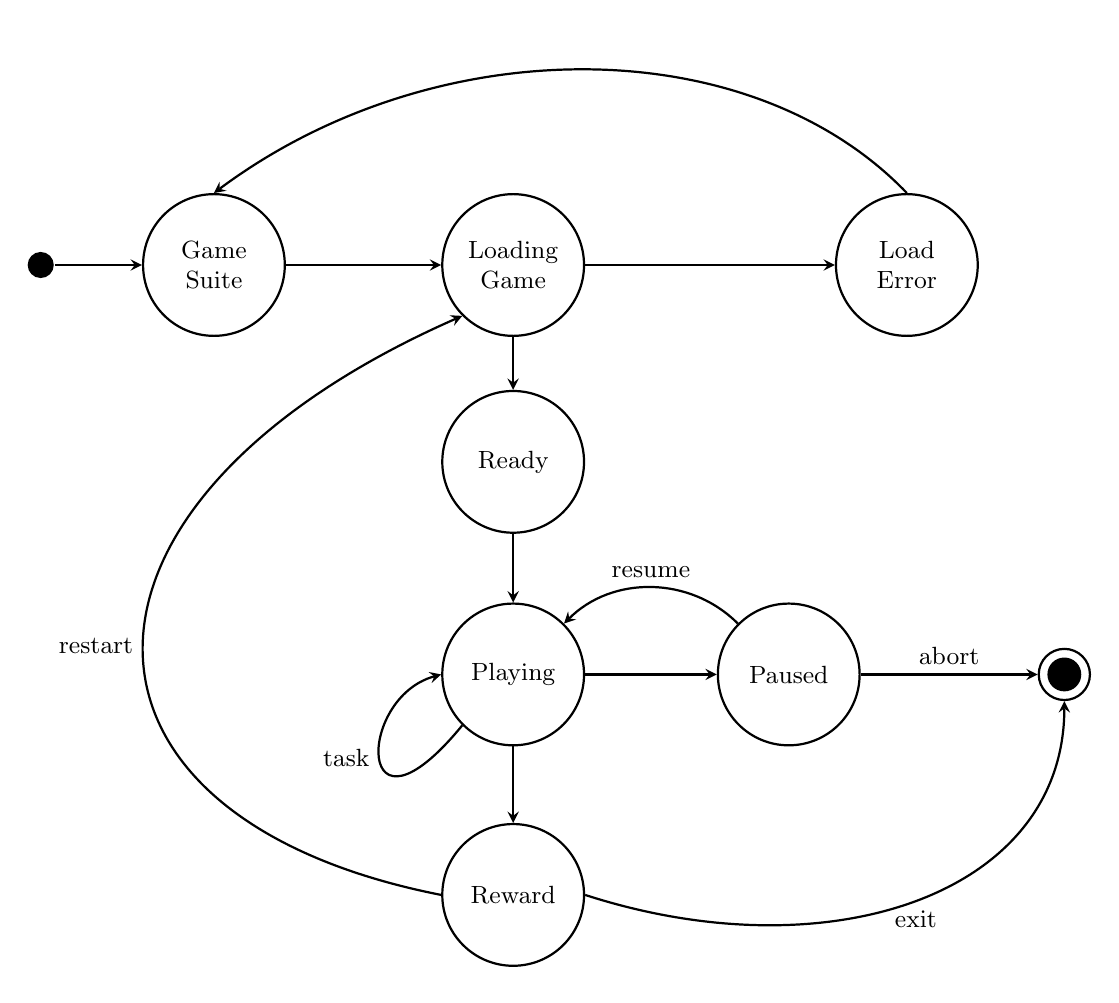
\begin{tikzpicture}[>=stealth,thick,
  state/.style={draw,circle,minimum size=1.8cm,align=center},
  every node/.style={font=\small}]
\node[circle,fill,minimum size=0.3cm] (start) at (-5,4) {};
\node[state] (suite) at (-2.8,4) {Game\\Suite};
\node[state] (loading) at (1,4) {Loading\\Game};
\node[state] (error) at (6,4) {Load\\Error};
\node[state] (ready) at (1,1.5) {Ready};
\node[state] (playing) at (1,-1.2) {Playing};
\node[state] (paused) at (4.5,-1.2) {Paused};
\node[state] (reward) at (1,-4) {Reward};
\node[draw,circle,minimum size=0.65cm] (end) at (8,-1.2) {};
\node[circle,fill,minimum size=0.43cm] at (end.center) {};
\draw[->] (start) -- (suite);
\draw[->] (suite) -- (loading);
\draw[->] (loading) -- (error);
\draw[->] (error.north) .. controls (4,7) and (0,7) .. (suite.north);
\draw[->] (loading) -- (ready);
\draw[->] (ready) -- (playing);
\draw[->] (playing) -- (paused);
\draw[->] (paused.north west) to[bend right=45]
  node[above] {resume} (playing.north east);
\draw[->] (playing.south west) .. controls (-1,-3.5) and (-1,-1.5) ..
  node[left] {task} (playing.west);
\draw[->] (playing) -- (reward);
\draw[->] (paused) -- node[above] {abort} (end);
\draw[->] (reward.east) .. controls (5,-5) and (8,-4) ..
  node[below] {exit} (end.south);
\draw[->] (reward.west) .. controls (-5,-3) and (-5,1) ..
  node[left] {restart} (loading.south west);
\end{tikzpicture}
